%!TEX root = ../main.tex
\chapter{相关工作综述}

\section{推荐系统的研究现状}

推荐算法的本质是通过一定方式将用户和物品联系起来,常用的方式有利用好友关系、用户的历史兴趣以及用户的注册信息等\cite{项亮2012推荐系统实践}。概括地说,推荐系统主要基于两种不同的方法或它们的组合:基于内容的方法和基于协同过滤的方法。

基于内容的推荐方法为用户和物品赋予简要的描述,以表示各自独特的性质,例如,电影的描述可以包括其类型、导演、票房等方面,用户的描述可以是个人资料或从已评分物品中识别出的共同特征,这样可以利用描述为用户匹配合适的物品。这种方式的好处很明显,透明度高,推荐方式直接,而且当有新物品出现时,利用物品的描述即可进行推荐。然而缺点也较为明显,基于内容的策略需要收集额外的信息,而这些信息可能并不容易得到,同时隐私问题也可能阻碍用户提供个人信息\cite{Koren2009Matrix}。

另一种策略,不像内容过滤那样需要明确的描述信息,而是围绕用户物品的评分矩阵,分析用户之间的关系和物品之间的相互依赖性,以获得新的用户和物品的关联,这种方法被称为协同过滤(Collaborative Filtering)\cite{Goldberg1992Using}。协同过滤算法是目前推荐系统研究的热点之一,大多数推荐算法都是在此基础上改进而来。传统的协同过滤仅利用评分信息进行推荐\cite{shi2014collaborative},主要分为两种类型,基于近邻的方法\cite{Desrosiers2011A,Sarwar2001Item,Deshpande2004Item}和基于潜在特征模型的方法\cite{xu2015ice}。前者直接利用存储在系统中的用户项目评分进行预测,因此又被称为基于存储的协同过滤。后者尝试从偏好度矩阵中推断出用户和物品的低维的特征向量映射,基于模型的方法具有良好的可扩展性和预测精确性而变得流行。传统的协同过滤克服了基于内容的一些限制,它比内容过滤的技术更加精确,但是却面临数据稀疏性和冷启动问题。因此,一些借助文本内容的信息的混合模型被提出来。

在协同过滤模型中引入内容信息是当今的研究热点之一,主题建模算法\cite{blei2009topic}用于从大量文档中发掘潜在的主题,主题模型提供了文档的低维表示\cite{Chang2009Reading},代表性的主题模型有隐式狄利克雷分布(LDA)\cite{Blei2003Latent},该模型的假设是文章与词之间是通过主题联系的。协同主题回归模型(CTR)\cite{Wang2011Collaborative}结合了基于潜在因素模型 \cite{Agarwal2009Regression,Salakhutdinov2007Probabilistic} 的协同过滤的思想和基于概率主题模型的内容分析\cite{Blei2003Latent,Chang2009Reading,Agarwal2010fLDA},使得系统在冷启动问题上表现良好。CTR-SMF \cite{purushotham2012collaborative} 以及 CTR-SMF2 \cite{chen2014context} 模型将社交信任矩阵引入 CTR 模型,以进一步提高推荐性能。


跨域推荐是一个新兴的研究课题,它旨在利用辅助域中的用户反馈来缓解目标域上的稀疏性问题\cite{hu2013personalized}。虽然跨域推荐的效果可能不如在单一域上的推荐准确,但跨域推荐将更加多样化,这可能对提高用户的满意度和参与度有好处。跨域推荐的关键挑战是在不同域的项目和用户之间发现有用的联系,通常所考虑的域之间看上去是不相关的,例如,音乐与感兴趣的地方,因此很难找到它们之间的关联\cite{shi2011tags},对于如何发掘不同域的信息产生了多种观点,例如,
Li 等人提出了基于迁移学习的方法\cite{li2009can},该方法将辅助域的稠密评分矩阵进行共现聚类并发掘每个类的评分模式,利用评分模式建立不同域之间的关联,在另外的工作中\cite{li2009transfer},假设用户和物品属于某个类服从概率分布,利用概率模型扩展了该方法。而基于连接的跨域模型利用标签或评论信息可以用于发掘不同域的用户或物品的兴趣\cite{kaminskas2011location,Enrich2013Cold,Xin2015Cross},因为不同域中用户产生的内容通常会具有关联。Zhuang \cite{zhuang2010cross} 等利用香农熵和逻辑回归进行一致性计算,从而建立不同域之间的关联。Cao \cite{cao2010transfer} 等提出一种概率贝叶斯框架解决了连接预测的问题,即预测在用户和物品之间的潜在连接。


标签系统的普及促进了推荐系统的发展,标签中蕴含着丰富的有价值的信息,用户用标签来描述对物品的看法,当一个用户为一些物品赋予了标签,那这些标签就反映了用户对物品的偏好\cite{chen2016capturing},如何利用标签数据提高个性化推荐的质量是推荐系统的重要课题\cite{项亮2012推荐系统实践}。目前,标签系统中主要有两种类型的协同过滤,标签推荐\cite{wang2013collaborative,fang2015personalized}的目的是为物品匹配合适的标签,另一种是基于标签的物品推荐\cite{zhou2010userrec,xu2011semrec},它旨在利用标签和评分等信息为目标用户推荐用户或物品。

\section{基于协同过滤的推荐系统}
协同过滤(Collaborative Filtering)是推荐系统中应用最早和最为成功的策略之一,这个术语最早由 David Goldberg 等人于 1992 年创造 ,用于描述一个实验性的邮件过滤系统 Tapestry \cite{Goldberg1992Using}。协同过滤克服了基于内容过滤的一些限制,它不使用内容信息,而是通过分析系统中其他用户和物品的评分信息,以获得新的用户和物品的关联。

随着互联网的不断发展,尤其是电子商务的出现,推荐算法随之快速发展,协同过滤在研究领域和实践中都去得了巨大成功,目前大部分推荐算法都是基于协同过滤算法改进而来,协同过滤的两个主要领域是基于近邻的方法和潜在因素模型。

\subsection{基于近邻的协同过滤}
最常见的协同过滤是基于近邻的方法,该方法的基本思想借鉴了人们生活中选择物品的方式,如果身边的朋友喜欢某件物品,那么自己就会有很大概率选择该物品。另外,如果用户喜欢某个物品,那么他很可能喜欢与该物品类似的物品。因此,该方法又分为基于用户的方法和基于物品的方法。

在基于近邻的协同过滤中,存储在系统中的用户项目评分直接用于预测新项目的评分,因此有被称为基于存储的协同过滤。该算法在用户评分矩阵并不稀疏的时候能够产生非常良好的效果,而且不需要训练,直接通过计算就可以给出推荐,但是当数据量非常庞大的时候,推荐过程伴随着大量的计算,这也从一定程度上阻碍该算法在线上系统当中的使用。

\subsubsection{基于用户的近邻推荐}
协同过滤最初的形式是以用户之间的关系为中心\cite{Desrosiers2011A},系统的实现分为两个阶段,首先在历史数据中发现那些具有相似品味的用户,然后利用邻居对物品 $i$ 的评分计算用户 $u$ 对一个新物品 $i$ 的评分 $r_{ui}$ 。假设我们计算得到了每个用户对 $u \neq v$ 之间的相似度 $w_{uv}$ ,与用户 $u$ 相似度最高的 $k$ 个用户的集合,称为 $u$ 的 $k$ 近邻($k$ -NN),该集合记为 $N(u)$。然而只有评价过物品 $i$ 的邻居才可以用来预测 $r_{ui}$ ,因此我们将这个邻居的集合记为  $N_i (u)$ ,可以用这些邻居对 $i$ 评分的平均值来估计  $r_{ui}$ :
\begin{equation}
\hat{r_{ui}} = \dfrac {1}  {| N_i (u) | }   \sum_{v \in  N_i (u)}{ r_{v,i} } .
\end{equation}

这个式子并没有考虑到邻居间可以具有不同相似度的问题,可以利用每一个邻居与 u 的相似度对评分加权平均。

\subsubsection{基于物品的协同过滤}
比较流行的是基于物品的方法\cite{Sarwar2001Item,linden2003amazon},基于用户的推荐依赖于“志同道合的用户”的观点,而基于物品的方法着重于相似物品的评分。为了使用相似性度量,首先确定 $u$ 选择过的与 $i$ 最相似的 $k$ 个物品,这 $k$ 个近邻的集合由 $N_u (i)$  表示,预测值 $r_{ui}$ 的计算方法是采用 $u$ 在集合 $N_u (i)$  中评分的加权平均:
\begin{equation}
\hat{r_{ui}} = \dfrac { \sum\limits_{j \in N_u (i)} w_{i,j} r_{u,j}}  {\sum\limits_{j \in N_u (i)} w_{i,j} } .
\end{equation}

\subsubsection{相似性权重计算}
构建基于近邻的推荐系统的最关键方面之一是相似性权重的计算,它对推荐系统的准确性和性能具有显著影响。相似性的计算基于这样的共识:相似的用户喜欢相似的物品,同时相似的物品被相似的用户喜欢。目前有多种方式用于相似性的计算,最常见的是将评分矩阵中的行列向量作为对应用户或物品的抽象,然后计算向量余弦夹角。实际上,当使用显式评分作为偏好度时,不同的用户往往会有差异,例如某些用户的评分普遍偏高,可以使用与评分平均值的偏移作为偏好度,因此,采用这种调整的余弦相似度,物品 $i$ 和 物品 $j$ 之间的相似度计算方法如下(以计算物品间相似性为例):
\begin{equation}
sim(i,j) = \dfrac{\sum\limits_{u \in U} (r_{u,i} - \bar{r_u})  (r_{u,j} - \bar{r_u})} {   \sqrt {\sum\limits_{u \in U}  {(r_{u,i} - \bar{r_u})}^2  }    \sqrt {\sum\limits_{u \in U}  {(r_{u,j} - \bar{r_u})}^2  }  } ,
\end{equation}
其中,$r_u$ 是用户 $u$ 评分的平均值。通常上不必考虑所有近邻,为相似度定义一个具体的最小阈值,或者将规模限制为一个固定值,而且只考虑 $k$ 个最近邻\cite{Jannach2010Recommender}。

\subsubsection{基于用户与物品方法对比}
应用基于近邻的协同过滤系统时,可以从以下几个方面考虑选择基于用户还是基于物品的方法\cite{Desrosiers2011A}:
\begin{enumerate}
	\item {准确性}:在电子商务系统中,用户的数量往往远大于商品的数量,数据的稀疏性会导致很难匹配到相似用户,因此推荐的精确性将收到严重影响,此时使用基于物品的方法会有更高的准确性。同样的,在用户数量少于物品的场景下,例如学术论文推荐系统,采用基于用户的方法会比较准确。

	\item {效率}:推荐算法的计算量和存储量也取决于用户和物品的比例,当用户量远超物品数量,计算用户之间的相似性会产生庞大的计算量,影响系统的可扩展性。因为用户只对少数物品评级,因此仅存储非零的或者前 $N$ 个相似性权重可以降低存储量和在线推荐的复杂度。

	\item {稳定性}:一般情况下系统中可用的物品与用户相比是更加静态的,因此物品相似性权重可以不用频繁地计算,这样,利用用户当前的数据可以进行实时的查询推荐,相比于基于用户的方法,系统具有更高的稳定性。

	\item {可辨识性}:面向物品的方法更适合解释推荐背后的原理,这是因为用户往往熟悉之前选择过的物品,而不知道那些所谓志同道合的用户。这样,可以向用户展示在当前预测中使用的邻居物品列表以及它们的相似性权重,通过修改列表或权重,用户可以交互的参与推荐过程。

\end{enumerate}


\subsection{基于潜在特征的协同过滤}
基于模型的方法不直接利用存储的评分进行预测,而是尝试从偏好度矩阵中推断出用户和物品的低维的特征向量映射,某种意义上,特征向量隐含了用户和物品在多个维度上的性质。在该模型中,用户对物品的预测偏好度是特征向量的线性结合。例如,每一个物品 $i$ 与向量 $q_i \in R^f$ 相关联,每一个用户 $u$ 与向量 $p_i \in R^f$ 相关联,它们的内积 $q_i^Tp_u$ 表现了用户 $u$ 对物品 $i$ 在 $f$ 个特征上的总体偏好度。 因此评分的估计由如下式子给出:
\begin{equation}
\hat{r_{ui}} = q_i^Tp_u.
\end{equation}
这种方法最主要的挑战是如何将每一个用户和物品映射到特征向量 $q_i, p_u \in R^f$ ,在完成了映射之后,推荐系统将很容易利用上面的公式预测用户对物品的评分。潜在特征向量映射的实现通常是基于矩阵分解的,奇异值分解(SVD)\cite{paterek2007improving}是一种最基本的矩阵分解算法,它的计算方式是使得到的矩阵与原始矩阵对应项的正则平方和误差最小:
\begin{equation}
\min_{q^*, p^*} {\sum\limits_{(u,i) \in \kappa} {{(r_{u,i}-q_i^Tp_u)}^2 + \lambda(||q_i||^2 + ||p_u||^2)} } ,
\end{equation}
这里,$\kappa$ 是训练集中所有已知评级的用户物品对 $(u,i)$ 的集合,系统通过拟合之前观测的样本来学习模型的参数,而我们的目标是预测未知的评分,所以应该通过正则化参数来避免过度拟合已知的项,常数 $\lambda$ 用于控制正则化的程度。

可以通过随机梯度下降算法(stochastic gradient descent)最小化上面的误差函数。首先通过求参数的偏导数找到函数的最速下降方向,然后不断迭代优化参数直至收敛。上面定义的函数里有两组参数 $p_{u}$ 和 $q_{i}$ ,对它们分别求偏导数,然后梯度相反的方向以 $\gamma$ 步长调整参数,可以得到如下的迭代公式:
\begin{equation}
\begin{aligned}
&q_i \leftarrow q_i + 𝛾 \cdot(e_{ui} \cdot p_u -\lambda \cdot q_i),\\
&p_u \leftarrow p_u + 𝛾 \cdot(e_{ui} \cdot q_i- \lambda \cdot p_u),
\end{aligned}
\end{equation}

样本数据中通常会存在用户和物品个体性的偏移,例如一些用户给分普遍偏高。因此,直接将 $q_i^Tp_u$ 视为最后的评分值是不明智的,可以为每个用户和物品设置偏移量,加入偏移后改写为如下形式:
\begin{equation}
\hat{r_{ui}} = \mu + b_i + b_u + q_i^Tp_u.
\end{equation}
其中,$\mu$ 是全部评分的平均值,参数 $b_i$ 和 $b_u$ 是在样本上用户 $u$ 和物品 $i$ 的偏移量。这样,观察到的评分被分为了四个组成部分:全局平均、用户偏移、物品偏移、用户物品匹配,这使得每一个部分可以单独解释其含义。



\section{概率主题模型}
主题建模算法用于从大量文档集合中发现一组主题,其中主题是关于词项的分布,主题模型提供了文档的低维表示\cite{Chang2009Reading},通常被用于语料库检索、文档分类和信息检索等任务。最常见的主题模型是隐式狄利克雷分布(LDA)\cite{Blei2003Latent},假设有 $K$ 个主题 $\beta_{1:k}$,每一个都是在固定词典上的分布。LDA 生成文档的大致流程如下:
对于语料库中的每一篇文档 $w_{jn}$ :
\begin{enumerate}
\item 从狄利克雷分布中选取主题分布 $\theta_j \sim Dirichlet(\alpha).$
\item 对于文档中的每一个词 $n$ :
	\begin{enumerate}
		\item 选取主题 $z_{jn} \sim Mult(\theta_j).$
		\item 选取单词 $w_{jn} \sim Mult(\beta_{z_{jn}}).$ 
	\end{enumerate}
\end{enumerate}
这个过程说明了文档中的每个词是如何从主题的集合中选取出来的:主题分布是文档特有的,但是主题的集合是整个语料库共享的。不像聚类模型那样每个文档只能属于一个类别,LDA 允许文档具有多个主题。
\begin{figure}[htbp]
\centering
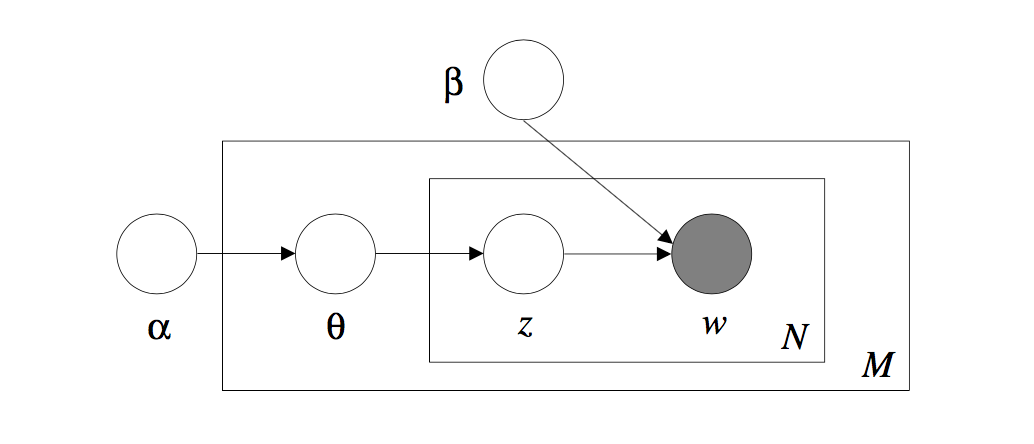
\includegraphics[width=0.7\linewidth]{images/lda.png}
\caption{LDA 的图模型。方框代表重复,外层的方框表示文档,而内层的方框表示文档中不断重复选择的主题和单词。}
\label{fig:fig1}
\end{figure}

LDA 属于非监督学习的范畴,给定一个文档语料库,我们可以使用变分 EM 算法来学习主题并根据它们给文档分配主题\cite{Blei2003Latent}。此外,给定一个新的文档,我们可以使用变分推理来确定其内容的主题。

矩阵分解的一个优点是它允许在特征向量中加入附加信息。Wang and Blei \cite{Wang2011Collaborative} 提出了协同主题回归模型(CTM)用于学术文章的推荐,该方法使用两种类型的数据:用户的收藏历史和文章的内容,结合了基于潜在因素模型 \cite{Agarwal2009Regression,Salakhutdinov2007Probabilistic} 的协同过滤的思想和基于概率主题模型的内容分析\cite{Blei2003Latent,Chang2009Reading}。模型很好的利用了内容信息,并将其结合到了传统的协同过滤算法中,使得系统在物品冷启动问题上表现良好。

\section{跨域推荐系统}
现有的推荐算法大多是仅针对属于单个域内的用户物品进行建模,因此是在单一域上的建模。事实上,用户在不同域中的偏好之间可能存在依赖性和相关性,例如,直观上来看,喜欢摇滚音乐的用户很可能喜欢科幻片,喜欢抒情音乐的用户或许喜欢爱情片。因此,在一个域中获得的用户兴趣特征可以在几个其他域中传递和利用,而不是独立地处理每种类型的项目。虽然跨域推荐的效果可能不如在单一域上的推荐准确,但跨域推荐将更加多样化,这可能对提高用户的满意度和参与度有好处 \cite{fernandez2012cross}。

Leizou \cite{Loizou2009How} 提出跨域推荐的三个主要研究趋势:
\begin{enumerate}
\item 通过集成和利用分布在不同系统中的显式用户偏好。
\item 通过记录用户的行为和反应来描述用户特征,并利用这些信息生成多个域上的推荐。
\item 通过组合来自不同域的推荐来生成单一域上的推荐。
\end{enumerate}

当两个域之间的用户和物品存在重叠时,我们可以直接将所有的信息看作属于一个共同的域,这样就可以利用传统的协同过滤进行跨域推荐。然而,当两个域没有重叠或重叠很小时,这种方法就会产生问题。为了解决上述不重叠的情况,我们必须找到某种方法,能够在域之间找到或建立某种类型的显式或隐式关系,其将被用作在推荐系统中连接不同域的桥梁\cite{fernandez2012cross}。

\subsection{基于迁移学习的模型}
迁移学习是机器学习领域的热门研究课题,基于迁移学习的跨域CF模型旨在通过对多个域的用户反馈建模来挖掘迁移模式,一种方法是在不同域中映射用户的特征向量,对于一个用户 $a$ ,假定他在目标域的特征向量是 $U_a$ ,辅助域中的为 $U'_a$ ,我们的目标是找到它们之间的映射函数,使得它们可以相互转换以提高两个域的效果。直观上,理想的情况是找到 $U_a$ 和 $U'_a$ 之间的可逆映射函数,但是有时候这种关系是非线性的,在这种情况下不能找到可逆函数 \cite{Xin2015Cross}。

在迁移学习的框架下,学习过程的每一次迭代,先利用随机梯度下降等算法更新单个域中的参数,然后利用域间的映射函数进行估计并得到误差,以最大后验概率的方式调整映射函数的参数。该方法的限制是需要依赖跨域共享的用户,即存在一些用户在多个域上都有行为数据。实际中,为了降低噪声干扰和复杂性,通常只利用那些在两个域都有密集活动的用户集合来训练模型。

\subsection{基于语义桥的跨域推荐}
基于连接的跨域协同过滤利用不同域间的具有相似内容的信息,将不同域间的物品连接起来。典型的方法是使用标签来桥接这些物品 \cite{Enrich2013Cold,chen2016capturing},因为不同域中使用的标签词汇之间的通常是重叠的\cite{项亮2012推荐系统实践},如果一个用户在辅助域中喜欢一个物品并赋予该物品某个标签,那么他也很可能喜欢目标域中具有相同标签的物品 \cite{Xin2015Cross}。例如,喜欢“romantic”电影的用户可能也喜欢“romantic”的书籍。

UserItemTags  \cite{shi2011tags}是一个结合标签的跨域推荐模型,它实现了在没有共享用户的情况下,利用辅助域信息缓解目标域的稀疏性问题。他们基于的假设是一个用户给一个物品的评分依赖于该用户赋予该物品的独特的标签,因此该模型在进行评分预测时,结合考虑目标用户赋予目标物品的标签。对于一个用户 $u$ ,一个物品 $i$ 和用户赋予物品的标签集合 $T_u(i)$ ,该算法依据如下规则预测评分:
\begin{equation}
\hat{r_{ui}} = p_u^T \cdot (q_i + \frac{1}{|T_u(i)|}  \sum\limits_{t  \in T_u(i)} {y_t}  ),
\end{equation}
其中,$p_u$,$q_i$ 和 $y_t$ 分别是用户 $u$、物品 $i$ 和标签 $t$ 的潜在特征向量。该模型参数的学习方法与 SVD 相同,采用随机梯度下降最小化正则平方误差,差别在于该模型同时遍历目标域和辅助域的评分和标签。

这个模型的主要限制是必须借助目标用户对目标物品的标签集合 $T_u(i)​$ ,而对于未被目标用户赋予标签的物品,则无法进行评分预测。本文在该模型的基础上进行改进,解决了上述限制,并挖掘了标签的主题,引入了语义信息,提高了推荐的效果。

\section{本章小结}

本章介绍了推荐系统目前的研究现状,从基本的协同过滤方法开始讨论,引出推荐系统中冷启动和稀疏性等关键的问题,并阐述了主题模型的思想,以及当今比较热门的跨域推荐的相关概念,内容基本涵盖了本文模型涉及到的相关技术。

本文的目标是将标签主题信息融入到传统的的协同过滤算法之中,提高单个域的推荐准确性,之后以标签主题的特征作为桥梁,引入跨域推荐的思想,从而在一定程度上缓解数据稀疏性问题。

